\exo{4}{Représenter} : Effectuer les conversions suivantes.

\begin{multicols}{4}
	\begin{enumerate}[label=\alph*.]
		\item $23~m^3$ en $dam^3$  \vspace*{13em}
		\item $0,12~km^3$ en $m^3$ \vspace*{13em}
		\item $43~L$ en $cm^3$ \vspace*{13em}
		\item $0,27~m^3$ en $dm^3$ \vspace*{13em}
	\end{enumerate}
\end{multicols}

\exo{4}{Modéliser} : 

On considère une boule de glace, de diamètre 6 cm dans un cornet de même diamètre et de hauteur 8 cm.

Si on laisse la glace fondre entièrement, est-ce qu'elle débordera du cornet ?

\newpage

\exo{4}{Calculer} : Calculer les aires des figures suivantes :

\begin{minipage}[t]{0.22\textwidth}
    \begin{figure}[H]
        \centering
        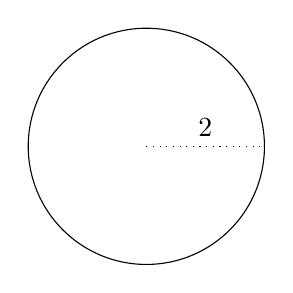
\begin{tikzpicture}
            \draw (0,0) circle (1.5);
            \draw[dotted] (0,0)--(1.5,0) node [midway, above] {2};
        \end{tikzpicture}
    \end{figure}
\end{minipage}
\hfill
\vrule
\hfill
\begin{minipage}[t]{0.22\textwidth}
    \begin{figure}[H]
        \centering
        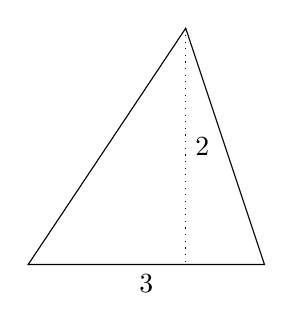
\begin{tikzpicture}
            \draw (0,0)--node[midway,below] {3} (3,0)--(2,3)--cycle;
            \draw [dotted] (2,3)--(2,0) node [midway, right] {2} ;
        \end{tikzpicture}
    \end{figure}
\end{minipage}
\hfill
\vrule
\hfill
\begin{minipage}[t]{0.22\textwidth}
    \begin{figure}[H]
        \centering
        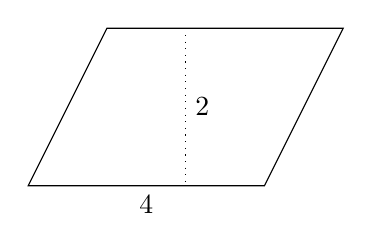
\begin{tikzpicture}
            \draw (0,0)--node [midway,below] {4} (3,0)-- (4,2)--(1,2)--cycle;
            \draw[dotted] (2,2)-- (2,0) node [midway,right] {2};
        \end{tikzpicture}
    \end{figure}
\end{minipage}
\hfill
\vrule
\hfill
\begin{minipage}[t]{0.22\textwidth}
    \begin{figure}[H]
        \centering
        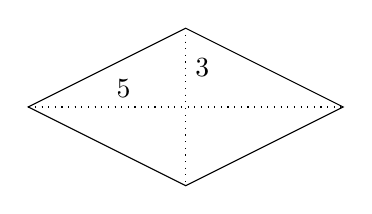
\begin{tikzpicture}
            \draw (0,0)-- (2,1)-- (4,0)--(2,-1)--cycle;
            \draw[dotted] (2,1)-- (2,0) node [midway,right] {3};
            \draw[dotted] (2,1)-- (2,-1) ;
            \draw[dotted] (0,0)-- (2,0) node [midway, above right] {5};
            \draw[dotted] (0,0)-- (4,0) ;
        \end{tikzpicture}
    \end{figure}
    \vspace{14em}
\end{minipage}

\exo{4}{Raisonner} : Calculer le volume des deux solides suivants.

\begin{minipage}[t]{0.45\textwidth}
    \begin{figure}[H]
        \centering
        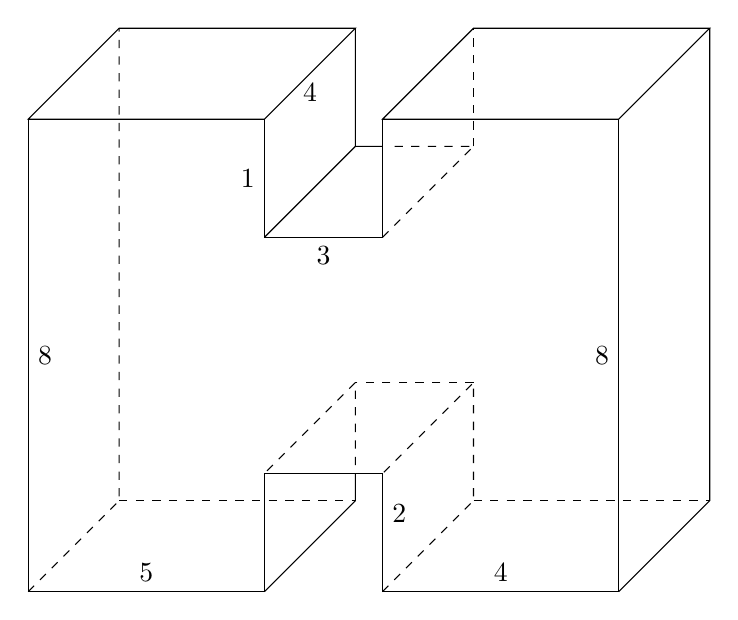
\begin{tikzpicture}[scale=1.5]
            \draw (0,4,0) --(2,4,0) -- node [midway,below] {4}  (2,4,-2) -- (0,4,-2)--cycle; %Face haute gauche
            \draw (3,4,0) --(5,4,0) -- (5,4,-2) -- (3,4,-2)--cycle; %Face haute droite
            \draw (5,0,0) -- (5,0,-2) -- (5,4,-2); %Cote droit
            \draw (2,0,0) -- (2,0,-2) -- (2,4,-2); %A faire en cavaliere
            \draw [fill=white] (2,3,0) --(2,3,-2) -- (3,3,-2)--(3,3,0); %Millieu haut
            \draw [fill=white] (0,0,0) --node [midway,above] {5} (2,0,0)-- (2,1,0)-- (3,1,0)-- node [midway,above right] {2} (3,0,0)--node [midway,above] {4} (5,0,0)--node [midway,left] {8}(5,4,0)--(3,4,0)-- (3,3,0)--node [midway,below] {3}(2,3,0) --node [midway,left] {1}(2,4,0)-- (0,4,0)--node[midway,right]{8} cycle; %Face avant
            \draw[dashed] (3,0,-2) --(5,0,-2);
            \draw[dashed] (3,0,0)--(3,0,-2)--(3,1,-2)--(3,1,0);
            \draw[dashed] (3,1,-2)--(2,1,-2);
            \draw[dashed] (0,0,-2) --(2,0,-2);
            \draw[dashed] (0,0,0)--(0,0,-2)--(0,4,-2);
            \draw[dashed] (2,0.3,-2)--(2,1,-2)--(2,1,0);
            \draw[dashed] (3,3,0)--(3,3,-2)--(2.3,3,-2);
            \draw[dashed] (3,3,-2)--(3,4,-2);
        \end{tikzpicture}
    \end{figure}
\end{minipage}
\hfill
\vrule
\hfill
\begin{minipage}[t]{0.45\textwidth}
    \begin{figure}[H]
        \centering
        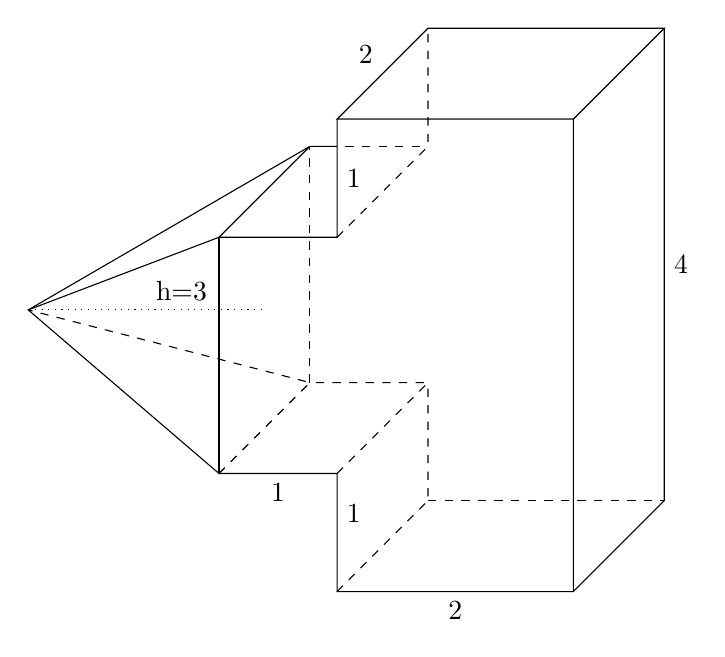
\begin{tikzpicture}[scale=1.5]
            \draw (3,4,0) --(5,4,0) -- (5,4,-2) -- (3,4,-2)-- node[midway,above left]{2} cycle; %Face haute droite
            \draw (5,0,0) -- (5,0,-2) -- node [midway,right] {4}(5,4,-2); %Cote droit
            \draw [fill=white] (2,3,0) --(2,3,-2) -- (3,3,-2)--(3,3,0); %Millieu haut
            \draw (2,3,-2)--(0,2,-1);
            \draw[fill=white] (0,2,-1)--(2,1,0)--node [midway,below] {1} (3,1,0)--node [midway,above right] {1} (3,0,0)--node [midway,below] {2} (5,0,0)--(5,4,0)--(3,4,0)--node [midway,right] {1}(3,3,0)--(2,3,0)--cycle; %Face avant
            \draw[dashed] (2,1,0)-- (2,1,-2)--(0,2,-1);
            \draw[dashed] (2,1,-2)--(2,3,-2);
            \draw (2,1,0)--(2,3,0);
            \draw[dashed] (3,0,-2) --(5,0,-2);
            \draw[dashed] (3,0,0)--(3,0,-2)--(3,1,-2);
            \draw[dotted] (0,2,-1)-- node [midway,above right]{h=3}(2,2,-1);
            \draw[dashed] (3,1,0)--(3,1,-2)--(2,1,-2);
            \draw[dashed] (3,3,0)--(3,3,-2)--(3,4,-2);
            \draw[dashed] (2.3,3,-2)--(3,3,-2);
        \end{tikzpicture}
    \end{figure}
    \vspace{15em}
\end{minipage}


